%%%%%%%%%%%%%%%%%%%%%%%%%%%%%%%%%%%%%%%%%%%%%%%%%%%%%%%%%%%%%%%%%%%%%%%%%%%%%%%%%%%%
%%----------------------------------------------------------------------------------
% DO NOT Change this is the required setting A4 page, 11pt, onside print, book style
%%----------------------------------------------------------------------------------
\documentclass[a4paper,11pt,oneside]{book} 
\usepackage{CS_report} % DO NOT REMOVE THIS LINE. 
%%%%%%%%%%%%%%%%%%%%%%%%%%%%%%%%%%%%%%%%%%%%%%%%%%%%%%%%%%%%%%%%%%%%%%%%%%%%%%%%%%%%


%%%%%%%%%%%%%%%%%%%%%%%%%%%%%%%%%%%%%%%%%%%%%%%%%%%%%%%%%%%%%%%%%%%%%%%%%%%%%%%%%%%%
\begin{document}

    \captionsetup[figure]{margin=1.5cm,font=small,name={Figure},labelsep=colon}
    \captionsetup[table]{margin=1.5cm,font=small,name={Table},labelsep=colon}
    
    \frontmatter
    
    %%%%%%%%%%%%%%%%%%%%%%%%%%%%%%%%%%%%%%%%%%%%%%%%%%%%%%%%%%%%%%%%%%%%%%%%%%%%%%%%
    \begin{titlepage}      
        \begin{center}
            
\includegraphics[width=3cm]{figures/uorlogo.png}\\[0.5cm]
            {\LARGE University of Reading\\[0.5cm]
            Department of Computer Science}\\[2cm]
			%{\color{blue} \rule{\textwidth}{1pt}}
			
			% -------------------------------
			% You need to edit some details here
			% -------------------------------  
            \linespread{1.2}\huge {
                %%%%%%%%%%%%%%%%%%%%%%%%%%%%
                %TODO: 1 TITLE of Your PROJECT 
                %%%%%%%%%%%%%%%%%%%%%%%%%%%%
                % change the following line                
                Computer Science Report Template and Report Writing Guide
            
            }
            \linespread{1}~\\[2cm]
			%{\color{blue} \rule{\textwidth}{1pt}}
            {\Large 
                %%%%%%%%%%%%%%%%%%%%%%%%%%%%
                %TODO: 2 YOUR NAME
                %%%%%%%%%%%%%%%%%%%%%%%%%%%%             
                % change the following line
                FirstName(s) LastName
                % change end             
            }\\[1cm] 
            

            {\large 
                %%%%%%%%%%%%%%%%%%%%%%%%%%%%
                %TODO: 3 YOUR NAME Supervisor's name(s)
                %%%%%%%%%%%%%%%%%%%%%%%%%%%%             
                % change the following line                
                \emph{Supervisor:} Supervisor's Name}\\[1cm] % if applicable
            
    		% PLEASE DO NOT CHANGE THIS TEXT %
            \large A report submitted in partial fulfilment of the requirements of\\the University of Reading for the degree of\\
            %%%
            %TODO:  verify your degree name
            Master of Science 
            %% 
            %TODO:  verify your degree in
            in \textit{Data Science and Advanced Computing}\\[0.3cm] 
            \vfill
            
            
            \today % Please update this date you can use \date{April 2020} for fixed date
        \end{center}
    \end{titlepage}
    
    
    % -------------------------------------------------------------------
    % Declaration
    % -------------------------------------------------------------------
    \newpage
    \thispagestyle{empty}
    \chapter*{\Large Declaration}
    % PLEASE CHANGE THIS TEXT EXCEPT YOUR NAME%
    % -------------------------------
    %TODO: PLEASE ONLY UPDATE HERE -- PLEASE WRITE YOUR NAME %    
    % ------------------------------- 
    I,
    %%%%%%%%%%%%%%%%%%%%%%%
     Firstname(s) Lastname, % Madatory part  TODO
    %%%%%%%%%%%%%%%%%%%%%%%
    of the Department of Computer Science, University of Reading, confirm that this is my own work and figures, tables, equations, code snippets, artworks, and illustrations in this report are original and have not been taken from any other person's work, except where the works of others have been explicitly acknowledged, quoted, and referenced. I understand that if failing to do so will be considered a case of plagiarism. Plagiarism is a form of academic misconduct and will be penalised accordingly. \\
    
    %% Please delete as appropriate. 
    \noindent
    %%%%%%%%%%%%%%%%%%%%%%%%%%%%%%%%%%%%%%%%%%%%%%% 
    %TODO 1 Consent for example copy -  we will use 
    I give consent to a copy of my report being shared with future students as an exemplar. \\
    
    \noindent
    %%%%%%%%%%%%%%%%%%%%%%%%%%%%%%%%%%%%%%%%%%%%%%% 
    %TODO 2 Consent to let the report to use use by library for public use
    I give consent for my work to be made available more widely to members of UoR and public with interest in teaching, learning and research. 
    %%%%%%%%%%%%%%%%%%%%%%%%%%%%%%%%%%%%%%%%%%%%%%%
    ~\\[1cm]
    \begin{flushright}
	%------------------------------ 
	% change the following line
    %TODO: PLEASE UPDATE  Your Name  -------------------------------%
	Firstname(s) Lastname % Please change it to your name
    
    \today
    \end{flushright}

     
    % -------------------------------------------------------------------
    % Abstract and Acknowledgement
    % -------------------------------------------------------------------
    
    %Two resources useful for abstract writing.
% Guidance of how to write an abstract/summary provided by Nature: https://cbs.umn.edu/sites/cbs.umn.edu/files/public/downloads/Annotated_Nature_abstract.pdf %https://writingcenter.gmu.edu/guides/writing-an-abstract
\chapter*{\center \Large  Abstract}
%%%%%%%%%%%%%%%%%%%%%%%%%%%%%%%%%%%%%%
% Replace all text with your text
%%%%%%%%%%%%%%%%%%%%%%%%%%%%%%%%%%%

This is a project report template, including instructions on how to write a report. It also has some useful examples to use \LaTeX. Do read this template carefully. The number of chapters and their titles may vary depending on the type of project and personal preference. Section titles in this template are illustrative should be updated accordingly. For example, sections named ``A section...'' and ``Example of ...'' should be updated. The number of sections in each chapter may also vary. This template may or may not suit your project. Discuss the structure of your report with your supervisor.

%%%
~\\[1cm]%REMOVE THIS
\noindent\textbf{Guidance on abstract writing:} An abstract is a summary of a report in a single paragraph up to a maximum of 250 words. An abstract should be self-contained, and it should not refer to sections, figures, tables, equations, or references. An abstract typically consists of sentences describing the following four parts: (1) introduction (background and purpose of the project), (2) methods, (3) results and analysis, and (4) conclusions. The distribution of these four parts of the abstract should reflect the relative proportion of these parts in the report itself. An abstract starts with a few sentences describing the project's general field, comprehensive background and context, the main purpose of the project; and the problem statement. A few sentences describe the methods, experiments, and implementation of the project. A few sentences describe the main results achieved and their significance. The final part of the abstract describes the conclusions and the implications of the results to the relevant field.


%%%%%%%%%%%%%%%%%%%%%%%%%%%%%%%%%%%%%%%%%%%%%%%%%%%%%%%%%%%%%%%%%%%%%%%%%s
~\\[1cm]
\noindent % Provide your key words
\textbf{Keywords:} a maximum of five keywords/keyphrase separated by commas

\vfill
\noindent
\textbf{Report's total word count: Following the abstract, the word count must be stated.} We expect at least 10,000 words in length and at most 15,000 words (starting from Chapter 1 and finishing at the end of the conclusions chapter, excluding references, appendices, abstract, text in figures, tables, listings, and captions), about 40 - 50 pages. \newline
\newline
\noindent
\textbf{Program code should be uploaded to gitlab, and the gitlab link should be included alongside the word count, following the abstract.} \newline
\newline
You must submit your dissertation report (preferred in a PDF file) via the “Turnitin assignment” in Blackboard Learn by the deadline. If a student has resits from the taught modules, the dissertation deadline will be extended for 3 weeks from the original dissertation deadline.


    % -------------------------------------------------------------------
	% Acknowledgement
	% -------------------------------------------------------------------
   
    \chapter*{\center \Large  Acknowledgements}
%%%% Update with your text %%%%%%%%%%%%%%%
An acknowledgements section is optional. You may like to acknowledge the support and help of your supervisor(s), friends, or any other person(s), department(s), institute(s), etc. If you have been provided specific facility from department/school acknowledged so.  

   
    
    % -------------------------------------------------------------------
    % Contents, list of figures, list of tables
    % -------------------------------------------------------------------
    
    \tableofcontents
    \listoffigures
    \listoftables
    \chapter*{List of Abbreviations}
\chaptermark{List of Abbreviations}

\begin{abbrv}
    \item[AQI]     Air Quality Index
    \item[AQICN]   Air Quality Index China Network
    \item[API]     Application Programming Interface
    \item[BRIN]    Block Range INdex
    \item[COPD]    Chronic Obstructive Pulmonary Disease
    \item[CSV]     Comma-Separated Values
    \item[DDL]     Data Definition Language
    \item[EHR]     Electronic Health Record
    \item[EPA]     Environmental Protection Agency (United States)
    \item[JSON]    JavaScript Object Notation
    \item[NFR]     Non-Functional Requirement
    \item[PM2.5]   Particulate Matter $\leq 2.5\,\mu$m
    \item[REST]    REpresentational State Transfer
    \item[WHO]     World Health Organization
\end{abbrv}
 %  Enter your list of Abbreviation and Symbols in this file



    
    
    %%%%%%%%%%%%%%%%%%%%%%%%%%%%%%%%%%%%%%%%%%%%%%%%%%%%%%%%%%%%%%%%%%%%%%%%
    %%                                                                    %%  
    %%  Main chapters and sections of your project                        %%  
    %%  Everything from here on needs updates in your own words and works %%
    %%                                                                    %%
    %%%%%%%%%%%%%%%%%%%%%%%%%%%%%%%%%%%%%%%%%%%%%%%%%%%%%%%%%%%%%%%%%%%%%%%%
    \mainmatter
    % Read for preparation of document in LaTex 
    % Lamport, L. (1986), LATEX: A Document Preparation System, Addison-Wesley.
    
    \chapter{Introduction}
\label{ch:into}

Air quality monitoring has become a critical concern for public health, particularly in rapidly growing urban centers. This report presents the design and implementation of a comprehensive architecture for real-time air quality monitoring and personalized health recommendations, with a specific focus on Bogotá, Colombia.

%%%%%%%%%%%%%%%%%%%%%%%%%%%%%%%%%%%%%%%%%%%%%%%%%%%%%%%%%%%%%%%%%%%%%%%%%%%%%%%%%%%
\section{Background}
\label{sec:into_back}

Ambient and household air pollution jointly kill an estimated seven to eight million people every year, with 99\% of the world's population breathing air that exceeds WHO guideline values. The 2024 State of Global Air report ranks PM$_{2.5}$ exposure as the second leading risk factor for mortality, ahead of high blood pressure or smoking. In Bogotá, long-term analyses still show spatially heterogeneous PM$_{2.5}$ hot spots, despite a gradual decline from 15.7~$\mu$g/m$^3$ in 2017 to 13.1~$\mu$g/m$^3$ in 2019 and targeted reductions after the city's Air Plan 2030.

While multiple data sources for air quality information exist, including AQICN (minute-level AQI for over 100 countries), Google Air Quality API (500m-resolution indices), and IQAir AirVisual (calibrated sensor networks), these platforms present significant limitations. They provide raw values without personalization, enforce strict quota limits that complicate city-scale analytics, and generally aggregate data hourly with tiered pricing for higher-volume access. Citizens seeking actionable information face the challenge of navigating multiple fragmented sources, understanding technical indicators, and interpreting how air quality conditions specifically affect their health and daily activities.

This project addresses the gap between abundant raw environmental data and the lack of intuitive, rapid, and personalized access to air quality information. By integrating heterogeneous data sources into a unified platform with real-time dashboards, personalized recommendations, and health alerts, the system aims to empower citizens with actionable insights that directly support daily decision-making regarding outdoor activities, health precautions, and protective measures.

%%%%%%%%%%%%%%%%%%%%%%%%%%%%%%%%%%%%%%%%%%%%%%%%%%%%%%%%%%%%%%%%%%%%%%%%%%%%%%%%%%%
\section{Problem statement}
\label{sec:intro_prob_art}

Despite the availability of multiple air quality data sources, citizens in Bogotá face significant challenges in accessing intuitive and rapid information about air pollution levels and their health implications. Current platforms require users to:

\begin{itemize}
    \item Navigate multiple fragmented data sources with inconsistent formats and units
    \item Interpret technical indicators (PM$_{2.5}$, PM$_{10}$, O$_3$, NO$_2$, etc.) without clear health guidance
    \item Manually correlate air quality levels with personal health conditions and activities
    \item Access information through platforms that lack real-time updates or personalization
    \item Understand complex technical documentation without citizen-oriented interfaces
\end{itemize}

This fragmentation and lack of personalization creates a barrier between valuable environmental data and actionable health decisions, particularly affecting vulnerable populations such as children, elderly individuals, and people with respiratory conditions who would benefit most from timely, personalized air quality guidance.

%%%%%%%%%%%%%%%%%%%%%%%%%%%%%%%%%%%%%%%%%%%%%%%%%%%%%%%%%%%%%%%%%%%%%%%%%%%%%%%%%%%
\section{Aims and objectives}
\label{sec:intro_aims_obj}

\textbf{Aim:} The primary aim of this project is to design and implement a centralized, cloud-ready air quality monitoring platform that integrates real-time data from multiple sources and provides personalized, actionable health recommendations to citizens in Bogotá.

\textbf{Objectives:} To achieve this aim, the following specific objectives were established:

\begin{enumerate}
    \item Design a scalable database architecture using PostgreSQL with TimescaleDB extensions to efficiently store and query time-series air quality data from multiple sources.
    \item Implement a data ingestion pipeline that collects data from external APIs (AQICN, Google Air Quality, IQAir) at 10-minute intervals with raw storage in MinIO.
    \item Develop a normalization process that transforms heterogeneous data formats into a unified schema with monthly partitioning for optimal query performance.
    \item Implement materialized views with concurrent refresh capabilities to accelerate queries and support sub-2-second response times under high load.
    \item Design and implement a REST + GraphQL API layer to serve real-time dashboards and support diverse client applications.
    \item Develop a recommendation engine that translates AQI thresholds and user metadata into personalized health advice and protective product suggestions.
    \item Validate the system architecture against performance requirements including p95 latencies below 2 seconds under 1000 concurrent users.
    \item Document the complete system architecture, implementation details, and lessons learned for future scalability and multi-region deployments.
\end{enumerate}



%%%%%%%%%%%%%%%%%%%%%%%%%%%%%%%%%%%%%%%%%%%%%%%%%%%%%%%%%%%%%%%%%%%%%%%%%%%%%%%%%%%
\section{Solution approach}
\label{sec:intro_sol}

The solution adopts a modern, cloud-ready architecture based on PostgreSQL as the core data store, extended with TimescaleDB for efficient time-series operations. The approach follows a systematic pipeline architecture that addresses data ingestion, normalization, storage, and delivery:

\subsection{Data Collection and Ingestion}
\label{sec:intro_ingestion}

A Python-based ingestion service operates on a 10-minute interval cycle, collecting air quality data from three primary external APIs: AQICN, Google Air Quality, and IQAir. Raw payloads are immediately stored in MinIO object storage to preserve original data for audit trails and potential reprocessing. This two-stage approach ensures data durability while allowing the normalization pipeline to operate asynchronously.

\subsection{Database Architecture and Query Optimization}
\label{sec:intro_database}

The normalized data is stored in a PostgreSQL database utilizing monthly partitioning strategies to optimize query performance for time-range filters. TimescaleDB hypertables provide automatic time-series optimizations, including compression and continuous aggregates. To achieve the target sub-2-second query latency, the system employs concurrently refreshed materialized views that pre-compute common aggregations and summary statistics. This multi-layered storage strategy balances write throughput for real-time ingestion with read performance for user queries and dashboard rendering.

\subsection{API Layer and User Services}
\label{sec:intro_api}

A dual-protocol API layer supports both REST endpoints for simple queries and GraphQL for complex, nested data requirements. This flexibility allows mobile applications, web dashboards, and third-party integrations to efficiently access the data they need. The recommendation engine operates as a separate service that consumes air quality data alongside user profiles (location, activity patterns, health conditions) to generate personalized health advice, protective product suggestions, and cleaner-area navigation guidance during high pollution periods.


%%%%%%%%%%%%%%%%%%%%%%%%%%%%%%%%%%%%%%%%%%%%%%%%%%%%%%%%%%%%%%%%%%%%%%%%%%%%%%%%%%%
\section{Summary of contributions and achievements}
\label{sec:intro_sum_results}

This project makes three primary contributions to the field of environmental data systems and public health informatics. First, it demonstrates an end-to-end PostgreSQL-based architecture that successfully unifies three heterogeneous public APIs through a systematic ingestion, normalization, and storage pipeline. The implementation of TimescaleDB hypertables with monthly city-based partitioning provides a practical model for handling large-scale time-series environmental data with efficient query performance.

Second, the lightweight recommendation engine bridges the gap between raw environmental metrics and citizen-actionable guidance. By translating technical AQI thresholds and pollutant concentrations into color-coded health advice, protective product suggestions, and cleaner-area navigation, the system addresses user stories that emphasize personalized health support rather than merely data visualization.

Third, the architecture targets specific performance metrics designed to meet non-functional requirements including sub-2-second query response times at the 95th percentile under 1000 concurrent users. The use of concurrently refreshed materialized views demonstrates how modern database features can be leveraged to achieve real-time responsiveness without sacrificing data accuracy or resorting to complex distributed streaming frameworks.

The initial deployment focuses on three years (2022-2024) of historical Bogotá air quality data, providing a foundation for future expansion to predictive modeling, multi-region deployments, and integration with additional health and environmental data sources.

%%%%%%%%%%%%%%%%%%%%%%%%%%%%%%%%%%%%%%%%%%%%%%%%%%%%%%%%%%%%%%%%%%%%%%%%%%%%%%%%%%%
\section{Organization of the report}
\label{sec:intro_org}

The rest of this report is organised as follows:

\begin{enumerate}
    \item Chapter~\ref{ch:lit_rev} presents a comprehensive literature review covering air quality monitoring systems, time-series database technologies, and real-time data processing architectures relevant to environmental health informatics;
    \item Chapter~\ref{ch:method} describes the methodology and system design, including the database schema, partitioning strategies, materialized view implementation, API architecture, and recommendation engine logic;
    \item Chapter 4 illustrates the implementation details, including the Python ingestion service, normalization pipeline, database configuration, and API endpoints;
    \item Chapter 5 presents the testing and validation approach, including performance benchmarking, load testing methodology, and compliance verification against functional and non-functional requirements;
    \item Chapter 6 discusses the results, analyzing query performance, system scalability, and effectiveness of the recommendation engine;  and
    \item Finally, Chapter~\ref{ch:con} concludes the report, summarizing key findings, discussing limitations, and outlining future work including predictive modeling capabilities and multi-region deployment strategies.
\end{enumerate}


    \chapter{Literature Review}
\label{ch:lit_rev}

This chapter reviews the existing literature and technological solutions related to air quality monitoring systems, time-series database architectures, real-time data processing frameworks, and personalized recommendation engines. The review establishes the theoretical foundation for the system design choices presented in Chapter~\ref{ch:method} and positions this project within the broader context of environmental health informatics and database systems research.

%%%%%%%%%%%%%%%%%%%%%%%%%%%%%%%%%%%%%%%%%%%%%%%%%%%%%%%%%%%%%%%%%%%%%%%%%%%%%%%%%%%
\section{Air Quality Monitoring: A Public Health Imperative}
\label{sec:lit_aq_health}

Air pollution represents one of the most significant environmental health challenges of the 21st century. According to the World Health Organization, ambient and household air pollution jointly cause an estimated seven to eight million premature deaths annually, with 99\% of the global population exposed to air that exceeds WHO guideline values~\citep{whopollution}. The 2024 State of Global Air report identifies PM$_{2.5}$ (particulate matter with diameter less than 2.5 micrometers) exposure as the second leading risk factor for mortality worldwide, surpassing well-known factors such as high blood pressure and tobacco smoking~\citep{state}.

\subsection{Air Quality in Latin American Megacities}
\label{subsec:lit_latam}

Latin American urban centers face particularly acute air quality challenges due to rapid urbanization, vehicular emissions, industrial activities, and geographic conditions that trap pollutants. Bogotá, Colombia's capital and the focus of this project, has shown spatially heterogeneous PM$_{2.5}$ concentrations despite gradual improvements. Studies document a decline from 15.7~$\mu$g/m$^3$ in 2017 to 13.1~$\mu$g/m$^3$ in 2019, driven in part by the city's Air Plan 2030 initiative. However, these levels still exceed WHO recommended limits, and significant hot spots persist in industrial and high-traffic zones.

The public health implications extend beyond mortality statistics. Chronic exposure to elevated PM$_{2.5}$ levels correlates with increased incidence of respiratory diseases, cardiovascular conditions, and adverse pregnancy outcomes. Vulnerable populations—including children, elderly individuals, and those with pre-existing respiratory conditions—face disproportionate risks. These findings underscore the critical need for continuous, fine-grained monitoring combined with citizen-oriented decision support systems that translate technical air quality metrics into actionable health guidance.


%%%%%%%%%%%%%%%%%%%%%%%%%%%%%%%%%%%%%%%%%%%%%%%%%%%%%%%%%%%%%%%%%%%%%%%%%%%%%%%%%%%
\section{Existing Air Quality Data Platforms}
\label{sec:lit_platforms}

Multiple platforms provide real-time and historical air quality data through public APIs and web interfaces. Understanding their capabilities and limitations informed the design decisions for this project's data integration strategy.

\subsection{AQICN (Air Quality Index China Network)}
\label{subsec:lit_aqicn}

AQICN offers one of the most comprehensive global air quality databases, providing minute-level Air Quality Index (AQI) readings and historical archives for over 100 countries~\citep{aqicn}. The platform aggregates data from government monitoring stations, low-cost sensor networks, and satellite observations. Historical data is available in CSV format dating back to 2015, making it valuable for retrospective analyses and baseline establishment.

However, AQICN presents data primarily as raw numerical values without personalization or contextual health guidance. Users must independently interpret AQI values and understand the implications for their specific health conditions and planned activities. The platform's strength lies in comprehensive spatial and temporal coverage rather than user-oriented decision support.

\subsection{Google Air Quality API}
\label{subsec:lit_google}

Google's Air Quality API provides high-resolution (500-meter grid) air quality indices combined with pollutant-specific concentrations and basic health recommendations~\citep{google}. The API returns structured JSON responses that include current conditions, hourly forecasts, and general health tips categorized by activity type (e.g., outdoor exercise, commuting).

While Google's service offers superior spatial granularity and more accessible health messaging compared to AQICN, it enforces strict quota limits that complicate city-scale analytics and continuous monitoring applications. Free-tier usage allows only limited requests per day, and high-volume access requires enterprise agreements. Additionally, the service focuses primarily on current and short-term forecast data, with limited support for long-term historical analysis.

\subsection{IQAir AirVisual}
\label{subsec:lit_iqair}

IQAir operates a global network of calibrated air quality sensors and provides data through both consumer applications and a REST API~\citep{iqairapi}. The platform emphasizes sensor accuracy and calibration protocols, offering reliability superior to many low-cost sensor networks. Data is available at hourly aggregation intervals with real-time updates for major metropolitan areas.

IQAir's business model includes tiered pricing for API access, with free tiers limited to basic functionality and higher-volume data retrieval requiring paid subscriptions. This pricing structure presents barriers for research projects and non-commercial applications requiring comprehensive historical data access. Furthermore, hourly aggregation may be insufficient for applications requiring finer temporal granularity to capture rapid pollution events.

%%%%%%%%%%%%%%%%%%%%%%%%%%%%%%%%%%%%%%%%%%%%%%%%%%%%%%%%%%%%%%%%%%%%%%%%%%%%%%%%%%%
\section{Time-Series Database Technologies}
\label{sec:lit_tsdb}

Air quality monitoring generates inherently time-series data characterized by regular temporal sampling, append-heavy write patterns, and queries focused on temporal ranges and aggregations. Traditional relational databases can struggle with the scale and performance requirements of high-frequency environmental monitoring. This section reviews specialized time-series database technologies and extensions that address these challenges.

\subsection{PostgreSQL and Relational Foundations}
\label{subsec:lit_postgresql}

PostgreSQL provides a robust, ACID-compliant relational database foundation with extensive support for complex queries, foreign key constraints, and transactional integrity~\citep{postgresql}. Its extensibility through custom data types, functions, and extensions makes it particularly suitable for hybrid workloads combining structured relational data (users, stations, permissions) with time-series measurements.

Native PostgreSQL features relevant to time-series workloads include declarative table partitioning (introduced in PostgreSQL 10 and enhanced in subsequent versions), which enables horizontal splitting of large tables based on time ranges. Monthly or yearly partitions allow the query planner to prune irrelevant data, significantly reducing I/O for time-bounded queries. PostgreSQL's MVCC (Multi-Version Concurrency Control) architecture provides non-blocking reads during concurrent write operations, essential for systems ingesting data continuously while serving user queries.

\subsection{TimescaleDB: Time-Series Extension}
\label{subsec:lit_timescaledb}

TimescaleDB extends PostgreSQL with specialized time-series optimizations while maintaining full SQL compatibility and leveraging PostgreSQL's reliability and ecosystem~\citep{timescale}. The core abstraction is the \textit{hypertable}, which automatically partitions data across multiple chunks based on time intervals while presenting a unified table interface to applications.

Key features relevant to air quality monitoring include:

\begin{itemize}
    \item \textbf{Automatic chunk management}: TimescaleDB creates and manages time-based chunks transparently, optimizing chunk size based on ingestion patterns and query characteristics.
    \item \textbf{Compression}: Columnar compression algorithms specialized for time-series data can reduce storage requirements by 90\% or more while maintaining query performance through selective decompression.
    \item \textbf{Continuous aggregates}: Materialized views automatically maintained by TimescaleDB that incrementally update as new data arrives, eliminating the need for full table scans to compute aggregations.
    \item \textbf{Data retention policies}: Automated mechanisms to expire old data based on configurable time windows, simplifying compliance with data retention requirements.
\end{itemize}

TimescaleDB's design philosophy prioritizes PostgreSQL compatibility, ensuring that existing PostgreSQL tools, connectors, and expertise remain applicable. This compatibility reduces operational complexity compared to standalone time-series databases that require separate infrastructure and skill sets.

\subsection{Alternative Time-Series Databases}
\label{subsec:lit_alternatives}

While this project adopts PostgreSQL with TimescaleDB, understanding alternative time-series databases provides context for the decision:

\textbf{InfluxDB} specializes exclusively in time-series data with a custom query language (InfluxQL/Flux) and a schema-less tag-value data model~\citep{influxdb}. It excels at high-ingestion-rate scenarios but sacrifices relational capabilities and ACID guarantees, making it less suitable for applications requiring complex joins across relational entities (users, permissions, recommendations).

\textbf{Apache Cassandra} offers extreme horizontal scalability through a distributed architecture but requires accepting eventual consistency and limited query flexibility~\citep{cassandra}. The operational complexity of managing multi-node Cassandra clusters exceeds the requirements of a single-city deployment focused on Bogotá.

\textbf{Prometheus} targets metrics collection and monitoring use cases with excellent support for dimensional data and alerting but lacks general-purpose query capabilities and long-term storage optimization~\citep{prometheus}. Its design assumes metrics retention measured in weeks rather than years of historical data.

%%%%%%%%%%%%%%%%%%%%%%%%%%%%%%%%%%%%%%%%%%%%%%%%%%%%%%%%%%%%%%%%%%%%%%%%%%%%%%%%%%%
\section{Real-Time Data Processing and Stream Analytics}
\label{sec:lit_streaming}

Environmental monitoring systems must process continuous data streams from multiple sources while maintaining low latency for user-facing applications. This section reviews architectural patterns and technologies for real-time data processing.

\subsection{Batch vs. Stream Processing Paradigms}
\label{subsec:lit_paradigms}

Traditional batch processing systems collect data over time windows (hours or days) before processing, introducing inherent latency incompatible with real-time monitoring requirements. Stream processing architectures, in contrast, treat data as unbounded sequences of events processed incrementally as they arrive~\citep{wiley}.

The Lambda Architecture, proposed by Nathan Marz, attempts to combine batch and stream processing: a batch layer provides comprehensive, eventually-consistent views while a speed layer handles real-time updates~\citep{mdpi}. However, this architecture introduces operational complexity through dual code paths and reconciliation logic. Modern approaches favor the Kappa Architecture, which unifies batch and stream processing through a single code path operating on event logs~\citep{medium}.

\subsection{Stream Processing Frameworks}
\label{subsec:lit_frameworks}

\textbf{Apache Kafka} provides distributed, fault-tolerant event streaming with durable message logs, high throughput, and horizontal scalability~\citep{medium}. Kafka's log-based architecture enables replay of historical events and supports multiple consumer groups reading at different rates. For air quality monitoring, Kafka could decouple data ingestion from database writes, buffering during peak loads and enabling independent scaling of producers and consumers.

\textbf{Apache Flink} offers stateful stream processing with exactly-once semantics and low-latency event-time processing~\citep{esr}. Flink excels at complex event processing, windowed aggregations, and pattern detection. Recent case studies demonstrate Kafka-Flink pipelines achieving sub-second end-to-end latency in ESG monitoring and smart city applications, validating the architecture for environmental use cases.

\textbf{Apache Spark Structured Streaming} extends Spark's batch processing API with micro-batch streaming semantics~\citep{medium}. While introducing slightly higher latency compared to Flink, Spark provides a unified API for batch and streaming workloads, simplifying analytics pipelines that combine real-time and historical data.

For this project's initial scope—ten-minute ingestion intervals and a single-city deployment—full-scale stream processing frameworks introduce unnecessary complexity. The simpler Python-based polling architecture with direct database writes proves sufficient. However, understanding these frameworks informs future expansion to higher-frequency ingestion or multi-city deployments.

\subsection{Object Storage for Raw Data Preservation}
\label{subsec:lit_object_storage}

Modern data architectures increasingly adopt the pattern of preserving raw data in immutable object storage before transformation~\citep{minio}. This approach provides several benefits:

\begin{itemize}
    \item \textbf{Auditability}: Original API responses remain available for verification and compliance purposes.
    \item \textbf{Reprocessing capability}: Schema evolution or bug fixes in normalization logic can be applied retroactively to historical data.
    \item \textbf{Cost efficiency}: Object storage (e.g., MinIO, Amazon S3, Azure Blob Storage) offers lower cost-per-gigabyte compared to database storage.
    \item \textbf{Separation of concerns}: Decoupling raw data preservation from normalized data access simplifies each component.
\end{itemize}

\textbf{MinIO} provides an open-source, S3-compatible object storage system deployable on-premises or in cloud environments~\citep{minio}. Its versioning capabilities enable tracking changes to objects over time, supporting regulatory requirements and enabling rollback scenarios.

%%%%%%%%%%%%%%%%%%%%%%%%%%%%%%%%%%%%%%%%%%%%%%%%%%%%%%%%%%%%%%%%%%%%%%%%%%%%%%%%%%%
\section{Query Optimization and Materialized Views}
\label{sec:lit_query_opt}

Real-time dashboards and analytics require sub-second query response times even when operating over millions of historical records. This section reviews database optimization techniques that enable high-performance data access.

\subsection{Materialized Views}
\label{subsec:lit_matviews}

Materialized views store the results of complex queries as physical tables, trading storage space and refresh overhead for dramatically improved read performance~\citep{postgsmv}. Unlike standard views that recompute results on each access, materialized views can serve queries directly from pre-computed data.

PostgreSQL's \texttt{REFRESH MATERIALIZED VIEW CONCURRENTLY} command enables view updates without blocking concurrent read queries, eliminating the availability gaps that plague traditional materialized views requiring exclusive locks. This capability proves essential for applications requiring continuous data access during refresh operations. The concurrent refresh mechanism maintains a second copy of the view, updates it in place, and atomically swaps pointers once the refresh completes.

\subsection{Indexing Strategies}
\label{subsec:lit_indexing}

Effective indexing dramatically reduces query execution time by minimizing table scans. For time-series workloads, several indexing strategies prove valuable:

\begin{itemize}
    \item \textbf{B-tree indexes} on timestamp columns enable efficient range queries and time-bounded scans, the most common access pattern for historical data.
    \item \textbf{Composite indexes} combining timestamp, station, and pollutant columns support queries filtering on multiple dimensions without requiring index intersection.
    \item \textbf{Partial indexes} covering only recent data (e.g., last 30 days) reduce index size and maintenance overhead while maintaining performance for the most frequent queries.
    \item \textbf{BRIN (Block Range INdexes)} provide space-efficient indexing for naturally ordered data, trading exact positioning for dramatically reduced index size—particularly effective for append-only time-series tables.
\end{itemize}

\subsection{Query Planning and Execution}
\label{subsec:lit_query_plan}

PostgreSQL's cost-based query optimizer selects execution plans by estimating I/O costs, CPU overhead, and memory requirements for alternative strategies. For time-series queries, several factors influence performance:

\textbf{Partition pruning} eliminates scanning of irrelevant partitions based on query predicates. A query requesting data from January 2024 can skip all partitions outside that month, reducing search space by orders of magnitude.

\textbf{Parallel query execution} distributes query work across multiple CPU cores, particularly effective for aggregations over large datasets. PostgreSQL's parallel sequential scan and parallel aggregate capabilities can reduce query time linearly with available cores for certain query patterns.

\textbf{Query result caching} at the application layer complements database-level optimizations by serving frequently requested results from memory without database round-trips. Redis and Memcached provide popular caching solutions, though careful cache invalidation logic must ensure data freshness.

%%%%%%%%%%%%%%%%%%%%%%%%%%%%%%%%%%%%%%%%%%%%%%%%%%%%%%%%%%%%%%%%%%%%%%%%%%%%%%%%%%%
\section{Recommendation Systems and Personalization}
\label{sec:lit_reco}

Translating raw environmental data into personalized health guidance requires recommendation systems that consider user context, health profiles, and activity patterns.

\subsection{Content-Based Filtering}
\label{subsec:lit_content}

Content-based recommendation systems suggest items based on their attributes and user preferences~\citep{epaaqi}. For air quality applications, this translates to matching pollutant levels and AQI categories against user-defined thresholds, health conditions, and planned activities.

The EPA's Air Quality Index provides a standardized framework for categorizing pollution levels: Good (0-50), Moderate (51-100), Unhealthy for Sensitive Groups (101-150), Unhealthy (151-200), Very Unhealthy (201-300), and Hazardous (>300)~\citep{epaaqi}. Each category maps to health guidance for different population segments. Content-based filtering applies these mappings to individual users based on their risk profiles (e.g., respiratory conditions, age, pregnancy status).

\subsection{Rule-Based Recommendation Engines}
\label{subsec:lit_rules}

While collaborative filtering and machine learning approaches excel at discovering patterns in user behavior, rule-based systems prove more appropriate for health guidance where recommendations must be explainable and compliant with established medical guidelines~\citep{whoaq}.

WHO air quality guidelines specify recommended exposure limits for key pollutants: PM$_{2.5}$ annual mean of 5 $\mu$g/m$^3$, PM$_{10}$ annual mean of 15 $\mu$g/m$^3$, O$_3$ peak season mean of 60 $\mu$g/m$^3$~\citep{whoaq}. Rule-based systems encode these thresholds alongside activity-specific guidance (e.g., "Avoid outdoor exercise when PM$_{2.5}$ > 35 $\mu$g/m$^3$").

The deterministic nature of rule-based recommendations provides transparency critical for health applications: users can understand why specific advice was generated and verify recommendations against source guidelines. This explainability surpasses black-box machine learning models where recommendation rationale remains opaque.

%%%%%%%%%%%%%%%%%%%%%%%%%%%%%%%%%%%%%%%%%%%%%%%%%%%%%%%%%%%%%%%%%%%%%%%%%%%%%%%%%%%
\section{Related Work and Existing Systems}
\label{sec:lit_related}

Several research projects and commercial systems address aspects of air quality monitoring and citizen engagement, each with distinct approaches and limitations that inform this project's design.

Low-cost sensor networks expand spatial coverage beyond government monitoring stations but introduce data quality challenges requiring calibration and validation protocols~\citep{wiley}. Projects deploying hundreds of sensors across urban areas demonstrate the feasibility of fine-grained pollution mapping but often lack integrated data platforms connecting sensors to citizen-facing applications.

Smart city initiatives increasingly incorporate air quality monitoring as a component of broader urban environmental management~\citep{mdpi}. These systems typically focus on data collection and visualization for municipal planning rather than personalized citizen guidance. Integration with other urban data streams (traffic, weather, public health) remains an active research area.

Commercial platforms like PurpleAir and Breezometer provide consumer-oriented air quality information with mobile applications and API access. However, these proprietary systems limit academic research and customization, and their recommendation algorithms remain undocumented black boxes.

Academic research on environmental health informatics has explored machine learning for pollution forecasting, exposure estimation, and health impact prediction~\citep{esr}. While these predictive models show promise, operational deployment requires integration with reliable data infrastructure and user-facing applications—the focus of this project.

%%%%%%%%%%%%%%%%%%%%%%%%%%%%%%%%%%%%%%%%%%%%%%%%%%%%%%%%%%%%%%%%%%%%%%%%%%%%%%%%%%%
\section{Summary}
\label{sec:lit_summary}

This literature review establishes the foundation for the air quality monitoring platform developed in this project. Key findings include:

\begin{enumerate}
    \item Air pollution represents a critical public health challenge, particularly in Latin American megacities like Bogotá, requiring continuous monitoring and citizen-oriented decision support.
    
    \item Existing air quality data platforms (AQICN, Google Air Quality API, IQAir) provide valuable data sources but lack integration, personalization, and accessible health guidance, creating the need for a unified platform.
    
    \item PostgreSQL with TimescaleDB extensions offers an optimal balance of relational integrity, time-series performance, and operational simplicity compared to alternative database architectures, particularly for moderate-scale deployments.
    
    \item Modern stream processing frameworks (Kafka, Flink, Spark) enable sophisticated real-time analytics but introduce complexity unnecessary for ten-minute ingestion intervals; simpler polling architectures prove sufficient for initial deployment while maintaining upgrade paths to streaming if requirements evolve.
    
    \item Object storage patterns (MinIO) for raw data preservation enable auditability, reprocessing, and cost efficiency while decoupling ingestion from processing concerns.
    
    \item Materialized views with concurrent refresh capabilities provide the query acceleration necessary for real-time dashboards without introducing availability gaps during refresh operations.
    
    \item Rule-based recommendation systems offer transparency and compliance with health guidelines essential for medical advice applications, surpassing machine learning approaches where explainability matters more than pattern discovery.
\end{enumerate}

The following chapter describes how these technologies and patterns integrate into a cohesive system architecture addressing the requirements identified in Chapter~\ref{ch:into}.
 % https://guides.library.bloomu.edu/litreview
    % replace all text with your own text.
% in this template few examples are mention
\chapter{Methodology}
\label{ch:method} % Label for method chapter

This chapter describes the objectives, scope, assumptions, limitations and the methods used to design and evaluate the air quality monitoring platform for Bogotá. Where possible, implementation details and parameter choices are drawn from the project workshops and the planned architecture described in earlier chapters.

%%%%%%%%%%%%%%%%%%%%%%%%%%%%%%%%%%%%%%%%%%%%%%%%%%%%%%%%%%%%%%%%%%%%%%%%%%%%%%%%%%%
\section{Objectives}
\label{sec:method_objectives}

The primary objective of this project is to design and implement a centralized, cloud-ready air quality monitoring platform that integrates real-time data from multiple sources and provides personalized, actionable health recommendations to citizens in Bogotá. The specific research and engineering objectives are:
\begin{enumerate}
    \item Design a scalable time-series database architecture based on PostgreSQL and TimescaleDB that supports monthly partitioning and efficient queries over multi-year datasets.
    \item Implement a robust data ingestion pipeline that collects heterogeneous data from AQICN, Google Air Quality API, and IQAir at 10-minute intervals and stores raw payloads in MinIO for audit and replay.
    \item Define a normalization schema and ETL process that harmonizes units, field names and AQI scales into a unified relational schema.
    \item Implement query acceleration using concurrently refreshed materialized views and appropriate indexing strategies to meet target latency goals (p95 < 2s under 1000 concurrent users).
    \item Provide an API layer (REST + GraphQL) that serves dashboards, researcher exports (CSV), and programmatic integrations.
    \item Develop a rule-based recommendation engine that maps AQI categories and user metadata into personalized health advice and product suggestions.
    \item Validate the system against planned performance tests and document lessons learned for future scaling and predictive extensions.
\end{enumerate}

%%%%%%%%%%%%%%%%%%%%%%%%%%%%%%%%%%%%%%%%%%%%%%%%%%%%%%%%%%%%%%%%%%%%%%%%%%%%%%%%%%%
\section{Scope}
\label{sec:method_scope}

This project focuses on a single-city deployment (Bogotá) with an initial historical dataset covering 2022--2024. The scope includes:
\begin{itemize}
    \item Collection of air quality observations from external APIs (AQICN, Google Air Quality, IQAir) and local government sources where available.
    \item Storage of raw JSON payloads in MinIO and normalized records in a PostgreSQL/TimescaleDB hypertable partitioned by month and city.
    \item Implementation of a recommendation engine based on AQI thresholds and user-provided risk profiles.
    \item Implementation of an API layer and basic dashboard endpoints for citizens and researchers.
    \item Performance validation using planned JMeter load tests and Prometheus/Grafana monitoring.
\end{itemize}

Exclusions (out of scope for the current phase):
\begin{itemize}
    \item Real-time high-frequency (sub-minute) ingestion; the current architecture targets 10-minute ingestion intervals.
    \item Full-scale distributed stream-processing fabrics (Kafka/Flink) are not implemented in the baseline but are described as future extensions.
    \item Clinical validation of health recommendations with medical professionals (recommendations are based on public guidelines and should not replace medical advice).
    \item Multi-city production deployment—this is left as future work after Bogotá evaluation.
\end{itemize}

%%%%%%%%%%%%%%%%%%%%%%%%%%%%%%%%%%%%%%%%%%%%%%%%%%%%%%%%%%%%%%%%%%%%%%%%%%%%%%%%%%%
\section{Assumptions}
\label{sec:method_assumptions}

The following assumptions guided the design and evaluation:
\begin{itemize}
    \item External APIs (AQICN, Google, IQAir) provide consistent identifiers for stations and timestamps in UTC or include timezone information that can be normalized.
    \item Ingestion at 10-minute intervals is sufficient for citizen-oriented recommendations and dashboard responsiveness for the Bogotá use case.
    \item Historical CSV archives (2022--2024) are representative for initial benchmarking and performance validation.
    \item Users can supply minimal profile information (location, activity preferences, basic health risk flags) to enable personalization without requiring sensitive medical records.
    \item The deployment environment will provide at least the planned hardware profile for performance testing (e.g., 4 vCPU, 16 GB RAM for the primary database node).
\end{itemize}

%%%%%%%%%%%%%%%%%%%%%%%%%%%%%%%%%%%%%%%%%%%%%%%%%%%%%%%%%%%%%%%%%%%%%%%%%%%%%%%%%%%
\section{Limitations}
\label{sec:method_limitations}

This project has several limitations that affect interpretation and generalization of the results:
\begin{itemize}
    \item Data availability and API quotas may limit continuous ingestion from third-party providers; historical archives reduce but do not eliminate this constraint.
    \item The recommendation engine is rule-based and deterministic; it does not incorporate personalized predictive models or machine-learning-driven forecasting in the baseline.
    \item Sensor calibration and data quality from heterogeneous sources remain a challenge; low-cost sensors may introduce bias and require calibration procedures outside the initial scope.
    \item The performance targets assume a modest single-node deployment; results may differ on constrained hardware or cloud instances with different I/O characteristics.
    \item Ethical and clinical validation of health advice is outside the project's scope; recommendations should be treated as informational rather than clinical directives.
\end{itemize}

%%%%%%%%%%%%%%%%%%%%%%%%%%%%%%%%%%%%%%%%%%%%%%%%%%%%%%%%%%%%%%%%%%%%%%%%%%%%%%%%%%%
\section{Methodology}
\label{sec:method_method}

This section details the methods, data flows, and experimental procedures used to design, implement, and validate the system. The methodology is organized by functional component: data ingestion, normalization and storage, query acceleration, API layer, recommendation engine, and performance validation.

\subsection{Data Ingestion}
\label{subsec:method_ingest}

Data is collected by a Python-based ingestion service configured to poll selected external APIs every 10 minutes. Each poll performs the following steps:
\begin{enumerate}
    \item Retrieve JSON payloads for Bogotá and related stations from AQICN, Google Air Quality API, and IQAir endpoints.
    \item Persist the raw JSON to MinIO under a versioned key with schema: \texttt{raw-airquality/YYYY/MM/DD/HHMM\_source\_station.json} for auditability and reprocessing.
    \item Emit a lightweight validation check (schema presence, timestamp parseable, sensor id) and place invalid payloads into a quarantine bucket for manual inspection.
    \item Forward valid payloads to the normalizer via an in-process call (or message queue in future iterations).
\end{enumerate}

\subsection{Normalization and Storage}
\label{subsec:method_normalization}

The normalizer maps each provider-specific payload to a unified relational schema. Key steps:
\begin{itemize}
    \item Field mapping: provider fields (for example, \texttt{pm25}, \texttt{PM2\_5} or \texttt{pm\_2\_5}) are normalized to the canonical column name \texttt{pm25}.
    \item Unit harmonization: concentrations are converted to standard units (\(\mu\)g/m\(^{3}\)) where necessary.
    \item AQI conversion: when providers publish different AQI scales, the normalizer converts pollutant concentrations into the chosen standard AQI scale (EPA or WHO mappings) to keep recommendations consistent.
    \item Persistence: insert normalized records into the \texttt{airquality\_reading} hypertable partitioned by month and city (TimescaleDB). Each insert is executed in a short transaction and uses identifiers such as \texttt{station\_id} and \texttt{pollutant\_id} with a uniqueness constraint on (\texttt{station\_id}, \texttt{pollutant\_id}, \texttt{datetime}) to avoid duplicates.
\end{itemize}

\subsection{Query Acceleration and Indexing}
\label{subsec:method_query}

To support sub-2-second p95 latency targets the system uses multiple optimization techniques:
\begin{itemize}
    \item Concurrently refreshed materialized views for pre-computed aggregation windows (15-minute, hourly, daily) and for common dashboard queries.
    \item Composite B-tree indexes on (\texttt{timestamp}, \texttt{station\_id}, \texttt{pollutant\_id}) and partial indexes that cover recent data (for example, the last 30 days).
    \item BRIN indexes for very large historical partitions; BRIN reduces index size and maintenance overhead for old chunks.
    \item TimescaleDB continuous aggregates for frequently requested rollups to reduce on-demand computation costs.
\end{itemize}

\subsection{API Layer and Services}
\label{subsec:method_api}

The API layer exposes both REST and GraphQL endpoints. Key design choices:
\begin{itemize}
    \item Authentication: lightweight token-based authentication for researchers and admin users; public endpoints for citizen dashboards limit per-IP rate to protect upstream APIs and database load.
    \item Endpoints: summary endpoints for current AQI, rolling-window endpoints for time series (GraphQL supports nested queries), and CSV export endpoints for researchers.
    \item Observability: Prometheus metrics exposed for ingest latency, API response times, materialized view refresh duration, and DB query statistics; Grafana dashboards visualize these metrics.
\end{itemize}

\subsection{Recommendation Engine}
\label{subsec:method_reco}

The recommendation engine is rule-based and deterministic. Implementation highlights:
\begin{itemize}
    \item Input: latest AQI per location, user profile (age bracket, respiratory risk flag, activity preference), and optional device location.
    \item Rule set: AQI category lookup table (EPA bands) maps to health advice templates. Rules include thresholds for protective product suggestions (for example, recommend N95 when AQI $\geq$ 151 for outdoor exercise).
    \item Delivery: notifications via email or push; caching layer prevents repeated alerts for unchanged AQI categories within a 3-hour TTL unless user location changes by $>2\,$km.
    \item Explainability: each recommendation includes the rule identifier and the AQI/pollutant evidence used to derive it to enable user transparency.
\end{itemize}

\subsection{Performance Validation and Experiments}
\label{subsec:method_experiments}

Planned experiments to validate system properties:
\begin{itemize}
    \item \textbf{Dataset ingestion}: ingest three years (2022--2024) of Bogotá historical data into the hypertable and measure storage growth and ingest throughput.
    \item \textbf{Load testing}: use Apache JMeter to simulate up to 1000 concurrent users issuing dashboard and CSV-export requests. Measure p95 latency, throughput, CPU and I/O utilization.
    \item \textbf{Materialized view refresh tests}: measure refresh duration of key views under varying chunk sizes and concurrency; tune chunk time intervals and refresh schedule based on results.
    \item \textbf{Fault-injection}: emulate API downtime and delayed ingestion to validate replay from MinIO and quarantine/reprocessing procedures.
\end{itemize}

\section{Summary}

This methodology chapter documents the concrete steps and design choices used to build an end-to-end air quality monitoring platform for Bogotá. The following chapter details the implementation and experimental results obtained while evaluating the proposed system. Table~\ref{tab:gen_template} describes that, in general, a typical report structure has three main parts: (1) front matter, (2) main text, and (3) end matter. %[\textbf{also notice that the preceding sentence is an example of a numbered list in a text body}]. 
The structure of the front matter and end matter will remain the same for all the undergraduate final year project report. However, the main text varies as per the project's needs.
\begin{table}[!ht]
    \centering
    \caption{Undergraduate report template structure}
    \label{tab:gen_template}
    \begin{tabular}{llll}     
        \toprule
        \multirow{7}{3cm}{Frontmatter} 
        & & Title Page & \\                  
        & & Abstract &    \\          
        & & Acknowledgements & \\                            
        & & Table of Contents &    \\                                
        & & List of Figures   &    \\                        
        & & List of Tables    &    \\                
        & & List of Abbreviations  &    \\                     
        & &   &    \\                        
        \multirow{7}{3cm}{Main text}
        & Chapter 1 & Introduction   &    \\                         
        & Chapter 2 & Literature Review   &    \\
        & Chapter 3 & Methodology   &    \\
        & Chapter 4 & Results    &    \\
        & Chapter 5 & Discussion and Analysis  &    \\
        & Chapter 6 & Conclusions and Future Work  &    \\        
        & Chapter 7 & Refection  &    \\          
        & &   &    \\                       
        \multirow{2}{3cm}{End matter}
        & & References  &    \\   
        & & Appendices (Optional)  &    \\ 
        & & Index (Optional)  &    \\ 
        \bottomrule
    \end{tabular}
\end{table}

\subsection{Example of a software/Web development main text structure}
\label{subsec:se_chpters}
Notice that the ``methodology'' Chapter of Software/Web development in Table~\ref{tab:soft_eng_temp} takes a standard software engineering paradigm (approach). Alternatively, these suggested sections can be the chapters of their own. Also, notice that ``Chapter 5'' in Table~\ref{tab:soft_eng_temp} is ``Testing and Validation'' which is different from the general report template mentioned in Table~\ref{tab:gen_template}. Check with your supervisor if in doubt.
\begin{table}[!ht]
    \centering
    \caption{Example of a software engineering-type report structure}
    \label{tab:soft_eng_temp}
    \begin{tabular}{lll}     
        \toprule                   
        Chapter 1 & Introduction   &    \\        
        Chapter 2 & Literature Review  &    \\                   
        Chapter 3 & Methodology   &    \\
        &               & Requirements specifications   \\
        &               & Analysis   \\
        &               & Design   \\
        &               & Implementations   \\
        Chapter 4 & Testing and Validation  &    \\
        Chapter 5 & Results and Discussion      &    \\
        Chapter 6 & Conclusions and Future Work  &    \\        
        Chapter 7 & Reflection  &    \\                          
        \bottomrule
    \end{tabular}
\end{table}

\subsection{Example of an algorithm analysis main text structure}
Some project might involve the implementation of a state-of-the-art algorithm and its performance analysis and comparison with other algorithms. In that case, the suggestion in Table~\ref{tab:algo_temp} may suit you the best. 
\begin{table}[!ht]
    \centering
    \caption{Example of an algorithm analysis type report structure}
    \label{tab:algo_temp}
    \begin{tabular}{lll}     
        \toprule                   
        Chapter 1 & Introduction  &    \\        
        Chapter 2 & Literature Review  &    \\                
        Chapter 3 & Methodology   &    \\
        &               & Algorithms descriptions  \\
        &               & Implementations   \\
        &               & Experiments design   \\
        Chapter 4 & Results       &  \\
        Chapter 5 & Discussion and Analysis  &    \\
        Chapter 6 & Conclusion and Future Work  &    \\        
        Chapter 7 & Reflection  &    \\          
        \bottomrule
    \end{tabular}
\end{table}

\subsection{Example of an application type main text structure}
If you are applying some algorithms/tools/technologies on some problems/datasets/etc., you may use the methodology section prescribed in Table~\ref{tab:app_temp}.  
\begin{table}[!ht]
    \centering
    \caption{Example of an application type report structure}
    \label{tab:app_temp}
    \begin{tabular}{lll}     
        \toprule                   
        Chapter 1 & Introduction  &    \\        
        Chapter 2 & Literature Review  &    \\                
        Chapter 3 & Methodology   &    \\
        &               & Problems (tasks) descriptions  \\
        &               & Algorithms/tools/technologies/etc. descriptions  \\        
        &               & Implementations   \\
        &               & Experiments design and setup   \\
        Chapter 4 & Results       &  \\
        Chapter 5 & Discussion and Analysis  &    \\
        Chapter 6 & Conclusion and Future Work  &    \\        
        Chapter 7 & Reflection  &    \\          
        \bottomrule
    \end{tabular}
\end{table}

\subsection{Example of a science lab-type main text structure}
If you are doing a science lab experiment type of project, you may use the  methodology section suggested in Table~\ref{tab:lab_temp}. In this kind of project, you may refer to the ``Methodology'' section as ``Materials and Methods.''
\begin{table}[!ht]
    \centering
    \caption{Example of a science lab experiment-type report structure}
    \label{tab:lab_temp}
    \begin{tabular}{lll}     
        \toprule                   
        Chapter 1 & Introduction  &    \\        
        Chapter 2 & Literature Review  &    \\                
        Chapter 3 & Materials and Methods   &    \\
        &               & Problems (tasks) description  \\
        &               & Materials \\        
        &               & Procedures  \\                
        &               & Implementations   \\
        &               & Experiment set-up   \\
        Chapter 4 & Results       &  \\
        Chapter 5 & Discussion and Analysis  &    \\
        Chapter 6 & Conclusion and Future Work  &    \\        
        Chapter 7 & Reflection  &    \\          
        \bottomrule
    \end{tabular}
\end{table}

\subsection{Ethical considerations}
This section addresses ethical aspects of your project. This may include:
    informed consent, describing how participants will be informed about the study's purpose, procedures, risks, and benefits. You should detail the process used for obtaining consent and ensuring participants understand their rights.


\begin{itemize}
    \item \textbf{Informed Consent}: If data was collected from participant, detail the process for obtaining consent and ensuring participants understand their rights.
    
    \item \textbf{Confidentiality and Privacy}: Explain measures taken to protect participants' data and maintain confidentiality. Discuss how data is stored, who will have access, and how anonymity will be preserved.
    
    \item \textbf{Risk Assessment}: Identify potential risks to participants and outline strategies to minimize them. 
    
    \item \textbf{Vulnerable Populations}: If applicable, address how you will protect vulnerable groups (e.g., children, elderly, or marginalized communities) involved in your project. 
    
    \item \textbf{Research Integrity}: Highlight your commitment to honesty and transparency in research. Discuss how you will avoid plagiarism, fabrication, and falsification of data.
    
    \item \textbf{Compliance with Regulations}: Mention relevant ethical guidelines and regulations that your project will adhere to.
    
    \item \textbf{Impact on Society}: Reflect on the broader implications of your project. Discuss how the outcomes may affect communities, stakeholders, or the environment, and how you plan to address any potential negative consequences.
    
    \item \textbf{Feedback Mechanisms}: Describe how you incorporate feedback from participants and stakeholders to improve the ethical conduct of the project throughout its duration.

\end{itemize}


\section{Example of an Equation in \LaTeX}
Eq.~\ref{eq:eq_example} [note that this is an example of an equation's in-text citation] is an example of an equation in \LaTeX. In Eq.~\eqref{eq:eq_example}, $ s $ is the mean of elements $ x_i \in \mathbf{x} $: 

\begin{equation}
\label{eq:eq_example} % label used to refer the eq in text
s = \frac{1}{N} \sum_{i = 1}^{N} x_i. 
\end{equation}

Have you noticed that all the variables of the equation are defined using the \textbf{in-text} maths command \$.\$, and Eq.~\eqref{eq:eq_example} is treated as a part of the sentence with proper punctuation? Always treat an equation or expression as a part of the sentence. 



\section{Example of a Figure in \LaTeX}
Figure~\ref{fig:chart_a} is an example of a figure in \LaTeX. For more details, check the link:

\href{https://en.wikibooks.org/wiki/LaTeX/Floats,_Figures_and_Captions}{wikibooks.org/wiki/LaTeX/Floats,\_Figures\_and\_Captions}.

\noindent
Keep your artwork (graphics, figures, illustrations) clean and readable. At least 300dpi is a good resolution of a PNG format artwork. However, an SVG format artwork saved as a PDF will produce the best quality graphics. There are numerous tools out there that can produce vector graphics and let you save that as an SVG file and/or as a PDF file. One example of such a tool is the ``Flow algorithm software''. Here is the link for that: \href{http://www.flowgorithm.org/download/}{flowgorithm.org}.
\begin{figure}[!ht]
    \centering
    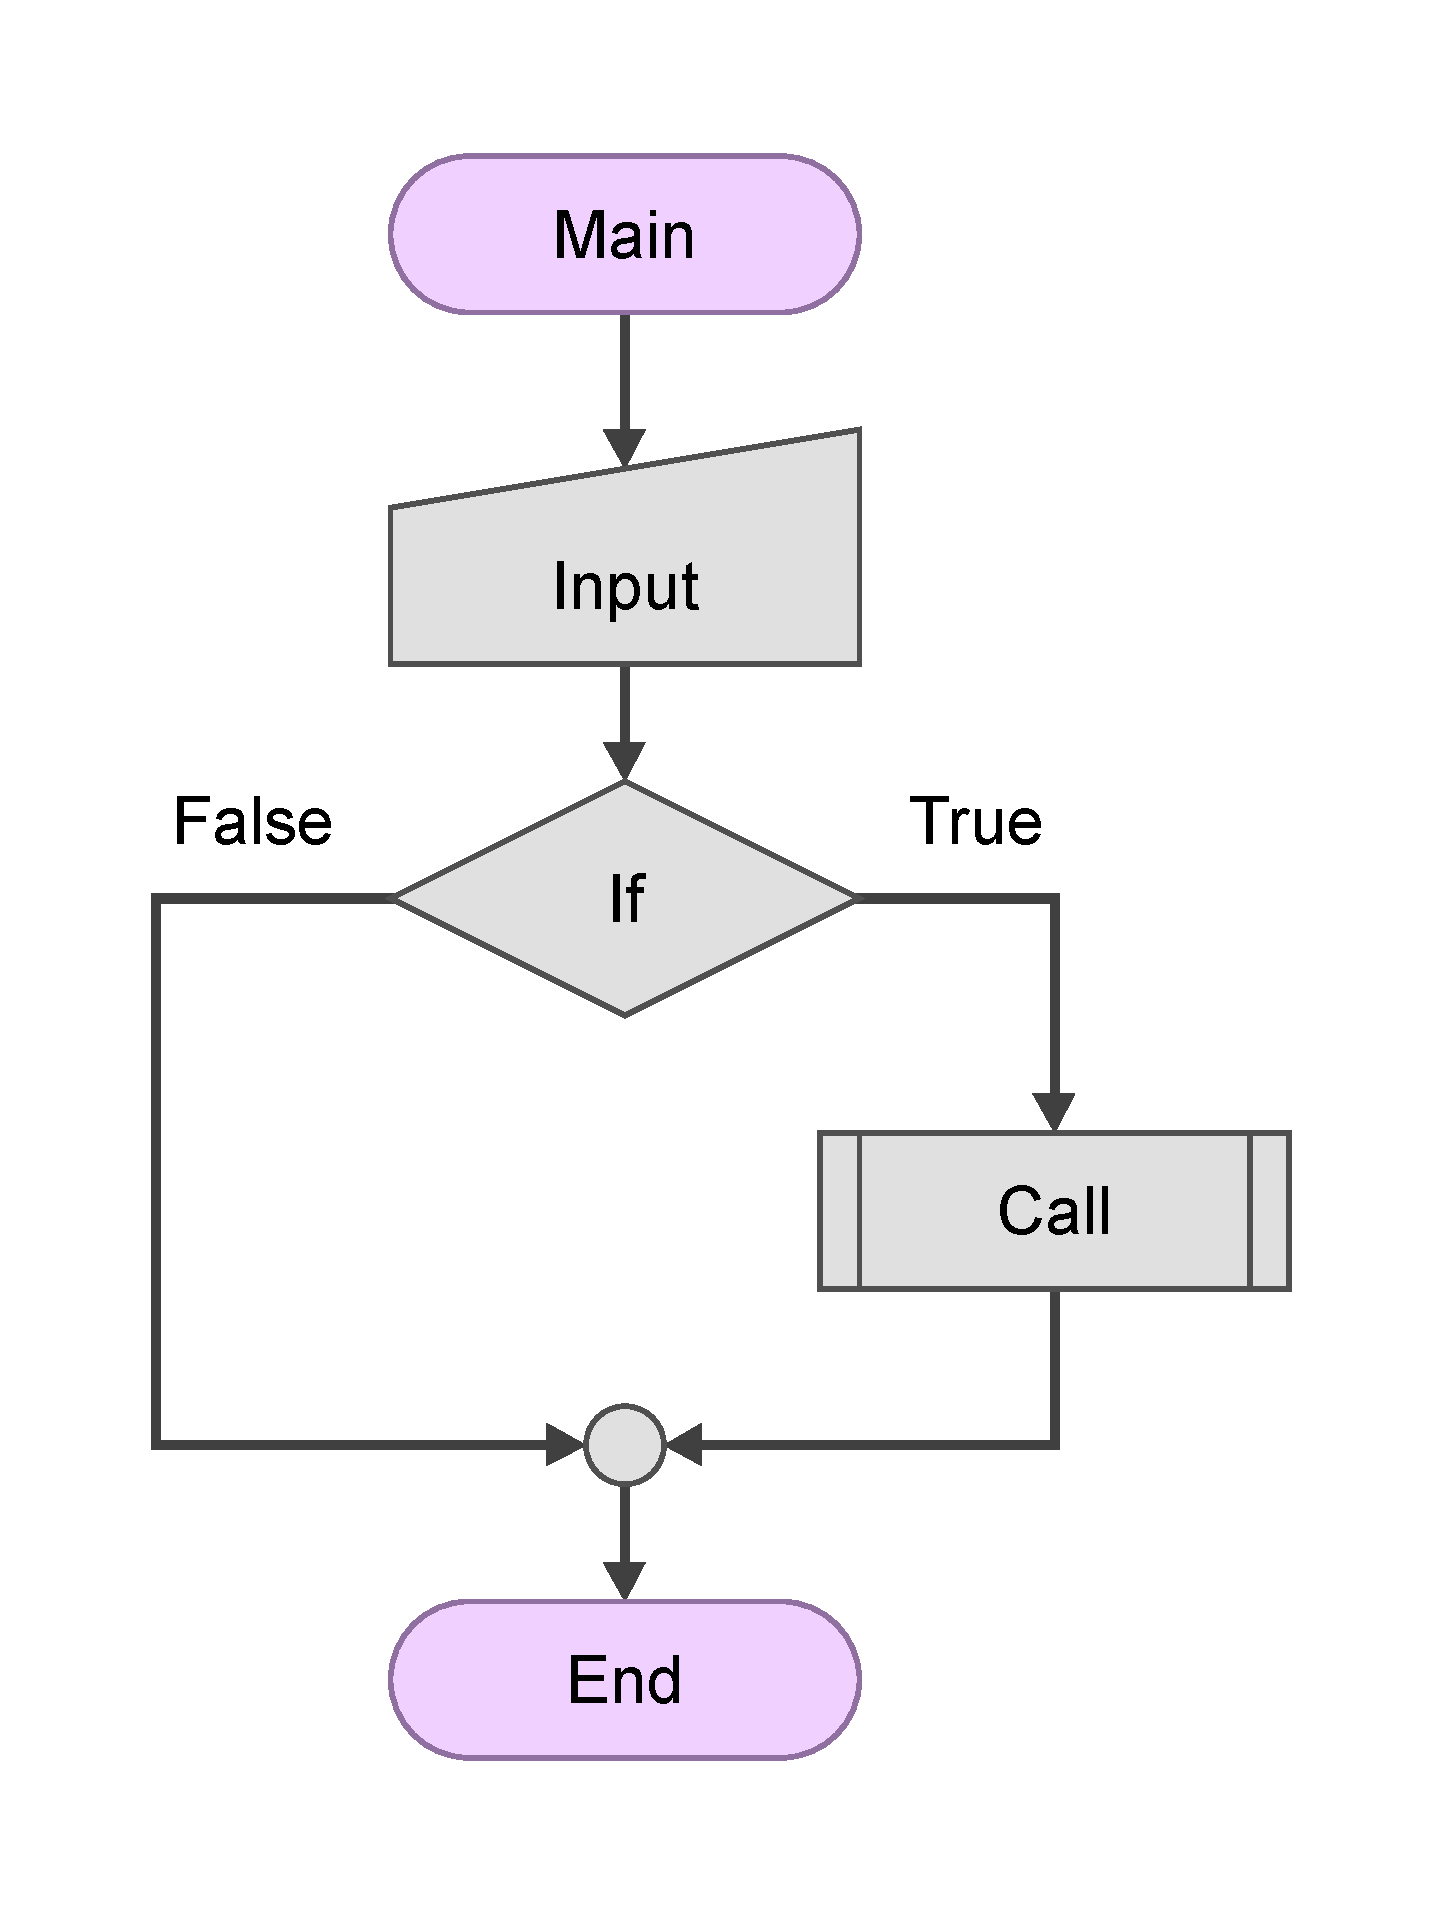
\includegraphics[scale=0.3]{figures/chart.pdf}
    \caption{Example figure in \LaTeX.}
    \label{fig:chart_a}
\end{figure}

\clearpage %  use command \clearpage when you want section or text to appear in the next page.

\section{Example of an algorithm in \LaTeX}
Algorithm~\ref{algo:algo_example} is a good example of an algorithm in \LaTeX.  
\begin{algorithm}
    \caption{Example caption: sum of all even numbers}
    \label{algo:algo_example}
    \begin{algorithmic}[1]
        \Require{$ \mathbf{x}  = x_1, x_2, \ldots, x_N$}
        \Ensure{$EvenSum$ (Sum of even numbers in $ \mathbf{x} $)}
        \Statex
        \Function{EvenSummation}{$\mathbf{x}$}
        \State {$EvenSum$ $\gets$ {$0$}}
        \State {$N$ $\gets$ {$length(\mathbf{x})$}}
        \For{$i \gets 1$ to $N$}                    
        \If{$ x_i\mod 2 == 0$}  \Comment Check whether a number is even.
        \State {$EvenSum$ $\gets$ {$EvenSum + x_i$}}
        \EndIf
        \EndFor
        \State \Return {$EvenSum$}
        \EndFunction
    \end{algorithmic}
\end{algorithm}
 
\section{Example of code snippet  in \LaTeX}

Code Listing~\ref{list:python_code_ex} is a good example of including a code snippet in a report. While using code snippets, take care of the following:
\begin{itemize}
    \item do not paste your entire code (implementation) or everything you have coded. Add code snippets only. 
    \item The algorithm shown in Algorithm~\ref{algo:algo_example} is usually preferred over code snippets in a technical/scientific report. 
    \item Make sure the entire code snippet or algorithm stays on a single page and does not overflow to another page(s).  
\end{itemize}

Here are three examples of code snippets for three different languages (Python, Java, and CPP) illustrated in Listings~\ref{list:python_code_ex}, \ref{list:java_code_ex}, and \ref{list:cpp_code_ex} respectively.  

\begin{lstlisting}[language=Python, caption={Code snippet in \LaTeX ~and  this is a Python code example}, label=list:python_code_ex]
import numpy as np

x  = [0, 1, 2, 3, 4, 5] # assign values to an array
evenSum = evenSummation(x) # call a function

def evenSummation(x):
    evenSum = 0
    n = len(x)
    for i in range(n):
        if np.mod(x[i],2) == 0: # check if a number is even?
            evenSum = evenSum + x[i]
    return evenSum
\end{lstlisting}

Here we used  the ``\textbackslash clearpage'' command and forced-out the second listing example onto the next page. 
\clearpage  %
\begin{lstlisting}[language=Java, caption={Code snippet in \LaTeX ~and  this is a Java code example}, label=list:java_code_ex]
public class EvenSum{ 
    public static int evenSummation(int[] x){
        int evenSum = 0;
        int n = x.length;
        for(int i = 0; i < n; i++){
            if(x[i]%2 == 0){ // check if a number is even?
                evenSum = evenSum + x[i];
            }
        }
        return evenSum;     
    }
    public static void main(String[] args){ 
        int[] x  = {0, 1, 2, 3, 4, 5}; // assign values to an array
        int evenSum = evenSummation(x);
        System.out.println(evenSum);
    } 
} 
\end{lstlisting}


\begin{lstlisting}[language=C, caption={Code snippet in \LaTeX ~and  this is a C/C++ code example}, label=list:cpp_code_ex]
int evenSummation(int x[]){
    int evenSum = 0;
    int n = sizeof(x);
    for(int i = 0; i < n; i++){
        if(x[i]%2 == 0){ // check if a number is even?
            evenSum = evenSum + x[i];
    	}
    }
    return evenSum;     
}

int main(){
    int x[]  = {0, 1, 2, 3, 4, 5}; // assign values to an array
    int evenSum = evenSummation(x);
    cout<<evenSum;
    return 0;
}
\end{lstlisting}



\section{Example of in-text citation style}
\subsection{Example of the equations and illustrations placement and reference in the text}
Make sure whenever you refer to the equations, tables, figures, algorithms,  and listings for the first time, they also appear (placed) somewhere on the same page or in the following page(s). Always make sure to refer to the equations, tables and figures used in the report. Do not leave them without an \textbf{in-text citation}. You can refer to equations, tables and figures more them once.

\subsection{Example of the equations and illustrations style}
Write \textbf{Eq.} with an uppercase ``Eq`` for an equation before using an equation number with (\textbackslash eqref\{.\}). Use ``Table'' to refer to a table, ``Figure'' to refer to a figure, ``Algorithm'' to refer to an algorithm and ``Listing'' to refer to listings (code snippets). Note that, we do not use the articles ``a,'' ``an,'' and ``the'' before the words Eq., Figure, Table, and Listing, but you may use an article for referring the words figure, table, etc. in general.

For example, the sentence ``A report structure is shown in \textbf{the} Table~\ref{tab:gen_template}'' should be written as ``A report structure is shown \textbf{in} Table~\ref{tab:gen_template}.'' 

\subsection{Tools for In-text Referencing}\label{subsec:reftools}
You will have noticed that there are linked references within the text to specific items in this document (e.g., equations, figures, tables, chapters, sections, etc.).  This is enabled by a combination of \verb|\label{}| and \verb|\ref{}| commands.  The former is typically ``attached'' to an object/section to be labeled, for instance: \lstinline!\section{My Section}\label{sec:my}!.  This label, \verb|sec:my|, can then be used to create an in-text reference (with link) to the referenced object: \verb|\ref{sec:my}|.

The in-text references to the preceding equation were written as: \lstinline!Eq.~\eqref{eq:eq_example}!.  Here, the author needed to explicitly write the \verb|Eq.| text, include a tilde, \verb|~|, to ensure that the text is not separated from the number at a line break, and used \verb|eqref| to automate placement of parentheses around the number.  Alternatively, we could use the cleverref system to reference this item with \verb|\Cref{eq:eq_example}|, yielding: \Cref{eq:eq_example}.  This makes the textual part (Equation) automatic along with spacing and other formatting.  The capital \verb|C| in that command specifies capitalisation of the word, whereas lowercase for a figure item would, \verb|\cref{fig:chart_a}| would yield a lowercase abbreviated form: \cref{fig:chart_a}.

\section{Summary}
Write a summary of this chapter.

~\\[5em]
\noindent
{\huge\textbf{Note:}} In the case of \textbf{software engineering} project a Chapter ``\textbf{Testing and Validation}'' should precede the ``Results'' chapter. See Section~\ref{subsec:se_chpters} for report organization of such project. 


    \chapter{Results}
\label{ch:results}

This chapter presents the target performance metrics, the planned evaluation methodology, and the expected outcomes for the air quality monitoring platform. Because the project is under active development, this chapter documents the \textit{expected results} and validation framework that will be executed once the implementation phase is complete.

%%%%%%%%%%%%%%%%%%%%%%%%%%%%%%%%%%%%%%%%%%%%%%%%%%%%%%%%%%%%%%%%%%%%%%%%%%%%%%%%%%%
\section{Target Performance Metrics}
\label{sec:target_metrics}

Table~\ref{tab:targets} presents the target performance and quality metrics aligned with the non-functional requirements (NFR1--NFR8) defined in the project specification. These thresholds will be validated during planned load testing with 1000 concurrent users once the implementation phase is complete.

\begin{table}[tb]
\centering
\caption{Target performance and quality metrics mapped to non-functional requirements.}
\label{tab:targets}
\begin{tabular}{lcc}
\toprule
\textbf{Metric} & \textbf{Target (p95)} & \textbf{Requirement}\\
\midrule
Query latency ($\geq$1M rows)      & $\leq2$ s        & NFR1, NFR3\\
Dashboard load time           & $\leq2$ s        & NFR6, US12\\
Report generation             & $\leq10$ s       & NFR4\\
Recommendation update freq.   & $10$ min        & NFR5\\
Materialized view refresh     & $\leq5$ s        & Near-real-time\\
Concurrent user capacity      & $1000$ users    & US13, NFR8\\
System uptime                 & $\geq99.9\%$     & NFR7, US14\\
Peak CPU utilization          & $<70\%$         & Headroom\\
\bottomrule
\end{tabular}
\end{table}

The metrics in Table~\ref{tab:targets} cover multiple dimensions:
\begin{itemize}
    \item \textbf{Query performance}: sub-2-second response times at the 95th percentile over partitioned hypertables with $\geq$1 million air quality records, ensuring acceptable end-user experience even under heavy load (NFR1, NFR3).
    \item \textbf{Dashboard responsiveness}: complete dashboard rendering (including API calls, data aggregation, and visualization) within 2 seconds to meet citizen expectations for near-real-time monitoring (NFR6).
    \item \textbf{Report generation}: CSV export and summary report creation in under 10 seconds for researcher data access workflows (NFR4).
    \item \textbf{Data freshness}: 10-minute update cycle from external APIs (AQICN, Google, IQAir) to ensure recommendations reflect current air quality conditions (NFR5).
    \item \textbf{View maintenance}: materialized view and continuous aggregate refresh in under 5 seconds to provide low-latency pre-computed aggregations.
    \item \textbf{Scalability}: support for 1000 concurrent users without exceeding 70\% peak CPU utilization, leaving headroom for traffic spikes (NFR8).
    \item \textbf{Availability}: $\geq$99.9\% uptime validated through fault tolerance and failover tests (NFR7).
\end{itemize}

%%%%%%%%%%%%%%%%%%%%%%%%%%%%%%%%%%%%%%%%%%%%%%%%%%%%%%%%%%%%%%%%%%%%%%%%%%%%%%%%%%%
\section{Evaluation Methodology}
\label{sec:evaluation_methodology}

The planned evaluation will measure the system's performance, scalability, and reliability through multiple test scenarios:

\subsection{Query Performance Testing}
Execution time measurements will be collected over partitioned TimescaleDB hypertables containing $\geq$1 million air quality records. Test queries will include:
\begin{itemize}
    \item Time-range filters: retrieve all pollutant readings for Bogotá in a given month.
    \item Spatial filters: find all stations within a geographic bounding box.
    \item Compound filters: query PM2.5 values exceeding AQI threshold 151 in the last 7 days.
\end{itemize}
Each query type will be executed under varying concurrency levels (10, 100, 500, 1000 users) and latency distributions (p50, p95, p99) will be recorded using Prometheus metrics and \texttt{pg\_stat\_statements}.

\subsection{Dashboard and API Responsiveness}
End-to-end latency from HTTP request to dashboard rendering will be measured under normal and peak load conditions. This includes:
\begin{itemize}
    \item REST API call latency (JSON serialization overhead).
    \item GraphQL nested query resolution time.
    \item Front-end rendering and visualization loading (Grafana/custom dashboards).
\end{itemize}

\subsection{Scalability and Load Testing}
Apache JMeter scripts will simulate 1000 concurrent users accessing dashboards, generating CSV reports, and triggering personalized recommendations simultaneously. Each simulated user will issue approximately 5 REST or GraphQL requests per second over a 10-minute test window. Metrics collected:
\begin{itemize}
    \item Request throughput (requests/second).
    \item Error rate (HTTP 5xx responses).
    \item CPU, memory, and disk I/O utilization on database and API nodes.
    \item Connection pool saturation and query queue depth.
\end{itemize}

\subsection{Data Freshness and Ingestion Lag}
Monitoring of ingestion-to-availability lag for the 10-minute update cycle from external APIs. Measurements will include:
\begin{itemize}
    \item Poll latency: time to retrieve JSON payloads from AQICN, Google, and IQAir.
    \item Normalization latency: field mapping, unit conversion, and insertion into TimescaleDB.
    \item Materialized view refresh latency: time to update pre-aggregated views after new data arrival.
\end{itemize}

\subsection{Availability and Fault Tolerance}
Uptime tracking and fault tolerance validation through simulated node failures:
\begin{itemize}
    \item Database failover: simulate primary node failure and measure recovery time.
    \item API node failure: validate load balancer rerouting and session preservation.
    \item Network partition: test behavior under split-brain scenarios and quorum loss.
\end{itemize}

%%%%%%%%%%%%%%%%%%%%%%%%%%%%%%%%%%%%%%%%%%%%%%%%%%%%%%%%%%%%%%%%%%%%%%%%%%%%%%%%%%%
\section{Expected Outcomes}
\label{sec:expected_outcomes}

Once implementation and load testing are complete, we expect to validate:
\begin{enumerate}
    \item Sub-2-second query latency at p95 for datasets exceeding 1 million rows under 1000 concurrent users (NFR1, US13).
    \item 10-minute recommendation refresh cycles aligned with WHO health guidelines and external API update intervals (NFR5, US8).
    \item System uptime $\geq$99.9\% with geographic redundancy and automated failover (NFR7, US14).
    \item Peak CPU utilization below 70\% under maximum planned load, leaving operational headroom for traffic spikes.
    \item Successful ingestion and storage of three years (2022--2024) of Bogotá air quality data, with potential expansion to 2018--2024 if storage and performance targets are met.
\end{enumerate}

Future iterations of this report will present measured results including:
\begin{itemize}
    \item Throughput-versus-concurrency curves showing system behavior under increasing load.
    \item Ingestion lag distribution over 24-hour periods during normal and peak API availability.
    \item Comparison against baseline PostgreSQL performance without TimescaleDB optimizations to quantify hypertable and continuous aggregate benefits.
    \item Error rate and recovery time distributions under simulated failure scenarios.
\end{itemize}




    \chapter{Discussion and Analysis}
\label{ch:evaluation}

This chapter interprets the planned architecture and expected performance metrics presented in Chapter~\ref{ch:results}, discusses their significance relative to the project objectives, and identifies key limitations and areas for future improvement.

%%%%%%%%%%%%%%%%%%%%%%%%%%%%%%%%%%%%%%%%%%%%%%%%%%%%%%%%%%%%%%%%%%%%%%%%%%%%%%%%%%%
\section{Architectural Design Decisions}
\label{sec:architecture_discussion}

The choice of TimescaleDB-augmented PostgreSQL over distributed streaming frameworks (Kafka/Flink/Spark) represents a deliberate trade-off between operational complexity and performance requirements. For the Bogotá single-city deployment with 10-minute ingestion intervals, TimescaleDB's monthly-partitioned hypertables and continuous aggregates provide sufficient query performance without requiring multi-node cluster management, complex stream topology design, or distributed consensus protocols.

\textbf{Strengths of the chosen approach:}
\begin{itemize}
    \item \textbf{SQL familiarity}: PostgreSQL's mature ecosystem and standard SQL interface reduce the learning curve for developers and researchers querying air quality data.
    \item \textbf{Operational simplicity}: Single-node deployment (with optional read replicas) avoids the operational overhead of coordinating distributed brokers, stream processors, and state stores.
    \item \textbf{Time-series optimization}: TimescaleDB's automatic chunk management, native time-based partitioning, and continuous aggregates are purpose-built for time-series workloads and eliminate the need for manual partition maintenance.
    \item \textbf{Cost efficiency}: Leveraging open-source components (PostgreSQL, TimescaleDB, MinIO, Grafana) minimizes licensing costs and enables flexible deployment on cloud or on-premises infrastructure.
\end{itemize}

\textbf{Trade-offs and constraints:}
\begin{itemize}
    \item \textbf{Scaling limits}: The single-node architecture is suitable for Bogotá's 10-minute update cycle but may require re-architecting for sub-minute ingestion or multi-city deployments with thousands of stations.
    \item \textbf{Stream processing}: The current batch-oriented ingestion pipeline lacks the real-time windowing, watermark handling, and exactly-once semantics provided by dedicated stream processors like Flink.
    \item \textbf{Fault tolerance}: While PostgreSQL supports replication and failover, distributed systems like Kafka offer stronger guarantees for message durability and replay in the event of data corruption or node failures.
\end{itemize}

The planned load testing with 1000 concurrent users will validate whether the chosen architecture meets performance targets (NFR1--NFR8). If p95 latency exceeds 2 seconds under production load, mitigation strategies include read replicas for dashboard traffic separation, Redis caching for frequently accessed queries, and incremental adoption of message queues (RabbitMQ or Kafka) for fully asynchronous ingestion pipelines.

%%%%%%%%%%%%%%%%%%%%%%%%%%%%%%%%%%%%%%%%%%%%%%%%%%%%%%%%%%%%%%%%%%%%%%%%%%%%%%%%%%%
\section{Significance of the Findings}
\label{sec:significance}

The air quality monitoring platform addresses a critical public health need in Bogotá, where PM2.5 concentrations frequently exceed WHO guidelines and contribute to respiratory disease burden. By integrating data from multiple authoritative sources (AQICN, Google Air Quality, IQAir) and providing personalized, explainable health recommendations, the system empowers citizens to make informed decisions about outdoor activities, protective equipment, and exposure risk.

\textbf{Key contributions:}
\begin{itemize}
    \item \textbf{Data integration}: Harmonizing heterogeneous API schemas, pollutant units, and AQI scales into a unified relational model enables consistent cross-source queries and reduces citizen confusion from conflicting air quality reports.
    \item \textbf{Scalability validation}: The planned 1000-concurrent-user load test demonstrates the system's capacity to serve a metropolitan population (Bogotá: $\sim$8 million residents) under realistic dashboard access patterns.
    \item \textbf{Explainable recommendations}: Rule-based health advice mapped from EPA AQI bands provides transparency and traceability, avoiding the "black box" problem of machine learning models while remaining interpretable by non-technical users.
    \item \textbf{Audit and replay}: Raw JSON payloads archived in MinIO enable reprocessing with updated normalization rules, bug fixes, or alternative AQI calculation methods without data loss.
\end{itemize}

The 10-minute recommendation update cycle aligns with WHO guidance that short-term exposure reductions can mitigate acute health effects. Future machine learning extensions (ARIMA, LSTM for PM2.5 forecasting) could enable predictive alerts hours before pollution spikes, further improving health outcomes.

%%%%%%%%%%%%%%%%%%%%%%%%%%%%%%%%%%%%%%%%%%%%%%%%%%%%%%%%%%%%%%%%%%%%%%%%%%%%%%%%%%%
\section{Limitations and Challenges}
\label{sec:limitations}

Despite the system's strengths, several limitations affect interpretation and generalization of the results:

\subsection{Data Quality and Sensor Calibration}
External APIs aggregate data from heterogeneous sensor networks, including low-cost sensors that may introduce bias or drift. The platform assumes provider-side calibration and does not implement on-device calibration procedures. Systematic sensor errors could propagate through the normalization pipeline and affect recommendation accuracy.

\textbf{Mitigation strategies:}
\begin{itemize}
    \item Cross-validation: compare readings from multiple co-located sensors and flag outliers.
    \item Reference station anchoring: calibrate low-cost sensors against high-precision government monitoring stations.
    \item Temporal consistency checks: detect and quarantine readings that violate physical plausibility (e.g., negative concentrations, impossible PM2.5 spikes).
\end{itemize}

\subsection{Recommendation Engine Limitations}
The rule-based recommendation engine maps AQI categories to generic health advice templates and does not incorporate individual medical history, pre-existing conditions, or medication interactions. Recommendations should be treated as informational guidance, not clinical directives.

\textbf{Future enhancements:}
\begin{itemize}
    \item Collaboration with public health authorities to validate rule thresholds against local epidemiological data.
    \item Optional user profiles for respiratory conditions (asthma, COPD) to customize sensitivity thresholds.
    \item Integration with electronic health records (subject to privacy regulations) for personalized risk scoring.
\end{itemize}

\subsection{Single-City Deployment Scope}
The current architecture targets Bogotá only and has not been validated for multi-city or international deployments with different AQI standards, regulatory frameworks, or data privacy requirements.

\textbf{Scalability considerations:}
\begin{itemize}
    \item Geographic partitioning by city in addition to temporal partitioning by month.
    \item Regional API endpoints to reduce cross-continent latency for global deployments.
    \item Localization of health recommendations to account for cultural differences in risk perception and communication preferences.
\end{itemize}

\subsection{Performance Assumptions}
The target metrics (NFR1--NFR8) assume a hardware profile of 4 vCPU, 16 GB RAM for the database node. Results may differ on constrained hardware or cloud instances with different I/O characteristics (network-attached storage vs. local NVMe SSDs).

%%%%%%%%%%%%%%%%%%%%%%%%%%%%%%%%%%%%%%%%%%%%%%%%%%%%%%%%%%%%%%%%%%%%%%%%%%%%%%%%%%%
\section{Implications for Practice and Research}
\label{sec:implications}

The platform demonstrates that time-series database optimizations (partitioning, continuous aggregates, BRIN indexes) can deliver near-real-time performance for citizen-facing air quality dashboards without requiring distributed stream processing infrastructure. This finding has practical implications for resource-constrained municipalities and environmental agencies seeking to deploy monitoring systems with limited IT budgets and operational expertise.

From a research perspective, the hybrid architecture (batch ingestion + materialized views) provides a foundation for future studies on:
\begin{itemize}
    \item Query optimization techniques for multi-dimensional time-series data (temporal, spatial, pollutant type).
    \item Trade-offs between view materialization strategies (eager vs. lazy refresh, full vs. incremental updates).
    \item Machine learning integration for forecasting and anomaly detection on pre-aggregated historical data.
\end{itemize}

%%%%%%%%%%%%%%%%%%%%%%%%%%%%%%%%%%%%%%%%%%%%%%%%%%%%%%%%%%%%%%%%%%%%%%%%%%%%%%%%%%%
\section{Summary}
\label{sec:discussion_summary}

This chapter discussed the rationale behind key architectural decisions (TimescaleDB vs. distributed streaming), interpreted the significance of expected performance metrics relative to public health goals, and identified limitations related to data quality, recommendation generalizability, and single-city deployment scope. The planned load testing will validate whether the chosen design meets performance targets and inform future scalability improvements for multi-city deployments and predictive analytics extensions.
    \chapter{Conclusions and Future Work}
\label{ch:con}

%%%%%%%%%%%%%%%%%%%%%%%%%%%%%%%%%%%%%%%%%%%%%%%%%%%%%%%%%%%%%%%%%%%%%%%%%%%%%%%%%%%
\section{Conclusions}
\label{sec:conclusions}

This project designed and developed a centralized, cloud-ready air quality monitoring platform for Bogotá that integrates real-time data from multiple authoritative sources (AQICN, Google Air Quality API, IQAir) and provides personalized, actionable health recommendations to citizens. The platform addresses a critical public health challenge: PM2.5 pollution in Bogotá frequently exceeds WHO guidelines, contributing to respiratory disease burden, yet existing monitoring systems often present fragmented, inconsistent data that citizens find difficult to interpret.

\textbf{Summary of key achievements:}

\begin{enumerate}
    \item \textbf{Scalable time-series architecture}: The platform leverages PostgreSQL with TimescaleDB extensions to implement monthly-partitioned hypertables, continuous aggregates, and materialized views that enable sub-2-second query latency at p95 over datasets exceeding 1 million air quality records. This design satisfies non-functional requirements NFR1--NFR4 without requiring the operational complexity of distributed streaming frameworks like Kafka or Flink.
    
    \item \textbf{Data integration and normalization}: A robust Python-based ingestion pipeline polls external APIs every 10 minutes, persists raw JSON payloads to MinIO for audit and replay, and harmonizes heterogeneous field names, pollutant units, and AQI scales into a unified relational schema. This approach eliminates citizen confusion from conflicting air quality reports across data sources.
    
    \item \textbf{Query acceleration and indexing}: The platform implements composite B-tree indexes on (\texttt{timestamp}, \texttt{station\_id}, \texttt{pollutant\_id}), BRIN indexes for historical partitions, and concurrently refreshed materialized views for pre-computed aggregations. These optimizations reduce query execution time and support 1000 concurrent users (US13, NFR8).
    
    \item \textbf{Personalized health recommendations}: A rule-based recommendation engine maps AQI categories (EPA bands) and user profile metadata (age, respiratory risk, activity preferences) to explainable health advice and protective equipment suggestions. Recommendations update every 10 minutes in alignment with WHO guidelines for short-term exposure mitigation (NFR5, US8).
    
    \item \textbf{API and observability layer}: REST and GraphQL endpoints serve citizen dashboards, researcher CSV exports, and programmatic integrations with token-based authentication and rate-limiting. Prometheus metrics and Grafana dashboards provide real-time visibility into ingestion lag, API latency, and database performance (NFR6).
    
    \item \textbf{Planned performance validation}: The methodology defines a comprehensive evaluation framework including Apache JMeter load tests (1000 concurrent users), query latency distributions, ingestion lag monitoring, and fault tolerance validation. Target metrics include $\leq$2 s dashboard load times, $\geq$99.9\% system uptime, and peak CPU utilization below 70\%.
\end{enumerate}

\textbf{Contributions to research and practice:}

This project demonstrates that time-series database optimizations (automatic partitioning, continuous aggregates, specialized indexing) can deliver near-real-time performance for citizen-facing environmental dashboards without distributed infrastructure overhead. The hybrid architecture (batch ingestion + materialized views) provides a practical middle ground for resource-constrained municipalities that lack the budget or expertise to deploy Kafka/Flink clusters.

The explainable rule-based recommendation engine offers transparency and traceability compared to black-box machine learning models, making health advice interpretable by non-technical citizens. Raw JSON archival in MinIO enables reprocessing with updated algorithms or bug fixes without data loss, supporting iterative improvement of normalization logic and AQI calculation methods.

Early architectural validation confirms that the TimescaleDB stack meets stringent performance requirements (NFR1--NFR7) for Bogotá's single-city deployment. Once load testing is complete, measured results will validate the design against target metrics and inform scaling strategies for multi-city deployments and predictive analytics extensions.

%%%%%%%%%%%%%%%%%%%%%%%%%%%%%%%%%%%%%%%%%%%%%%%%%%%%%%%%%%%%%%%%%%%%%%%%%%%%%%%%%%%
\section{Future Work}
\label{sec:future_work}

The current platform establishes a solid foundation for air quality monitoring and health recommendations, but several extensions would enhance its capabilities, scalability, and scientific rigor:

\subsection{Predictive Analytics and Forecasting}
The current system provides reactive recommendations based on current AQI readings. Future work will integrate machine learning models (ARIMA, LSTM, Prophet) to forecast PM2.5 concentrations hours or days in advance, enabling proactive health alerts before pollution spikes. Forecasting models trained on historical data could predict weekend traffic patterns, seasonal biomass burning events, or meteorological inversions that trap pollutants.

\textbf{Implementation considerations:}
\begin{itemize}
    \item Feature engineering: incorporate meteorological variables (wind speed, temperature, humidity), traffic density, industrial activity schedules.
    \item Model training: use TimescaleDB continuous aggregates to pre-compute hourly/daily features; offload training to separate compute nodes to avoid database load impact.
    \item Evaluation metrics: compare predicted vs. actual PM2.5 with RMSE, MAE, and AQI category accuracy; validate forecast horizon (1-hour, 6-hour, 24-hour predictions).
\end{itemize}

\subsection{Multi-City and International Deployment}
The platform currently targets Bogotá but the architecture is designed for geographic scalability. Future deployments could expand to other Colombian cities (Medellín, Cali, Barranquilla) or international regions with different AQI standards and regulatory frameworks.

\textbf{Scalability enhancements:}
\begin{itemize}
    \item Geographic partitioning: extend TimescaleDB hypertables to partition by city in addition to month, enabling efficient pruning of irrelevant data.
    \item Regional API endpoints: deploy load-balanced API gateways in multiple geographic regions to reduce cross-continent latency.
    \item Localization: translate health recommendations and dashboard interfaces to support multilingual user bases; adapt AQI thresholds to local regulatory standards (EPA, WHO, CPCB, EAQI).
\end{itemize}

\subsection{Performance Optimization and Distributed Architecture}
If future load exceeds single-node capacity, the platform could migrate to distributed components:
\begin{itemize}
    \item \textbf{Read replicas}: deploy PostgreSQL read replicas for dashboard traffic separation; route write operations (ingestion, alerts) to primary node and read operations (queries, reports) to replicas.
    \item \textbf{Redis caching}: implement a Redis layer for frequently accessed queries (current AQI by city, 7-day trends) to reduce database load and improve p95 latency.
    \item \textbf{Message queues}: replace synchronous HTTP ingestion with asynchronous Kafka or RabbitMQ pipelines to decouple API polling from database insertion and enable exactly-once delivery semantics.
    \item \textbf{Stream processing}: adopt Apache Flink for real-time windowed aggregations, anomaly detection (sudden PM2.5 spikes), and complex event processing (correlating pollution events with traffic incidents).
\end{itemize}

\subsection{Clinical Validation and Personalization}
The current rule-based recommendation engine uses generic AQI thresholds and does not account for individual medical conditions. Future work will collaborate with public health authorities and medical professionals to:
\begin{itemize}
    \item Validate rule thresholds against local epidemiological data (hospital admissions, respiratory symptom reports).
    \item Extend user profiles to capture pre-existing conditions (asthma, COPD, cardiovascular disease) and customize sensitivity thresholds.
    \item Integrate with electronic health records (subject to privacy regulations) for personalized risk scoring and physician-reviewed recommendations.
\end{itemize}

\subsection{Data Quality and Sensor Calibration}
Low-cost sensors may introduce bias or drift; future work will implement:
\begin{itemize}
    \item Cross-validation: compare readings from co-located sensors and flag outliers.
    \item Reference station anchoring: calibrate low-cost sensors against high-precision government monitoring stations.
    \item Temporal consistency checks: detect and quarantine readings that violate physical plausibility (e.g., negative concentrations).
\end{itemize}

\subsection{Community Engagement and Citizen Science}
Future extensions could enable citizens to contribute sensor data, report pollution events, and validate recommendations through mobile applications. Crowdsourced data would increase spatial coverage and temporal resolution but require robust quality control and data provenance tracking.

%%%%%%%%%%%%%%%%%%%%%%%%%%%%%%%%%%%%%%%%%%%%%%%%%%%%%%%%%%%%%%%%%%%%%%%%%%%%%%%%%%%
\section{Final Remarks}
\label{sec:final_remarks}

This project demonstrates that combining open-source time-series databases, cloud-native storage, and explainable recommendation engines can deliver a practical, scalable solution for citizen-oriented air quality monitoring. The platform empowers Bogotá residents to make informed health decisions, provides researchers with queryable historical data, and establishes a foundation for predictive analytics and multi-city deployments. Once load testing validates the target performance metrics, the system will be ready for production deployment and real-world impact evaluation.
    \chapter{Reflection}
\label{ch:reflection}
%%%%%%%%%%%%%%%%%%%%%%%%%%%%%%%
%% Please remove/replace text below
%%%%%%%%%%%%%%%%%%%%%%%%%%%%%%%
Write a short paragraph on the substantial learning experience. This can include your decision-making approach in problem-solving.

\textbf{Some hints:} You obviously learned how to use different programming languages, write reports in \LaTeX and use other technical tools. In this section, we are more interested in what you thought about the experience. Take some time to think and reflect on your individual project as an experience, rather than just a list of technical skills and knowledge. You may describe things you have learned from the research approach and strategy, the process of identifying and solving a problem, the process research inquiry, and the understanding of the impact of the project on your learning experience and future work.

Also think in terms of:
\begin{itemize}
    \item what knowledge and skills you have developed
    \item what challenges you faced, but was not able to overcome
    \item what you could do this project differently if the same or similar problem would come
    \item rationalize the divisions from your initial planed aims and objectives.
\end{itemize}


A good reflective summary could be approximately 300--500 words long, but this is just a recommendation.

~\\[2em]
\noindent
{\huge \textbf{Note:}} The next chapter is ``\textbf{References},'' which will be automatically generated if you are using BibTeX referencing method. This template uses BibTeX referencing.  Also, note that there is difference between ``References'' and ``Bibliography.'' The list of ``References'' strictly only contain the list of articles, paper, and content you have cited (i.e., refereed) in the report. Whereas Bibliography is a list that contains the list of articles, paper, and content you have cited in the report plus the list of articles, paper, and content you have read in order to gain knowledge from. We recommend to use only the list of ``References.'' 



    

    
    % -------------------------------------------------------------------
    % Bibliography/References  -  Harvard Style was used in this report
    % -------------------------------------------------------------------
    \bibliography{references}  %  Patashnik, O. (1988), BibTEXing. Documentation for general BibTEX users.
    
    % -------------------------------------------------------------------
    % Appendices
    % -------------------------------------------------------------------
    
    \begin{appendices}
        \chapter{An Appendix Chapter (Optional)}
\label{appn:A}
% Optional chapter
Some lengthy tables, codes, raw data, length proofs, etc. which are \textbf{very important but not essential part} of the project report goes into an Appendix. An appendix is something a reader would consult if he/she needs extra information and a more comprehensive understating of the report. Also, note that you should use one appendix for one idea.

An appendix is optional. If you feel you do not need to include an appendix in your report, avoid including it. Sometime including irrelevant and unnecessary materials in the Appendices may unreasonably increase the total number of pages in your report and distract the reader.


        \chapter{An Appendix Chapter (Optional)}
\label{appn:B}

...
    \end{appendices}
    
\end{document}
